\subsubsection{Why the Thermodynamic Cost of Erasing History
Matters}\label{why-the-thermodynamic-cost-of-erasing-history-matters}

I want readers to understand something that many academic circles are
only beginning to explore: erasing history is not just a moral or
cultural loss --- it is a calculable act of destruction. There is a
\emph{cost} associated with it. And that cost is not only societal or
ideological. It is physical. It is thermodynamic.

This idea struck me deeply one morning, after an overnight reflection on
a study I conducted last spring. Drawing from Shannon entropy, Huffman
coding, and Rolf Landauer's thermodynamic theory of information, I
realized that every attempt to delete a fact --- to erase even a single
\emph{bit} of truth --- carries an irreversible energy cost. This isn't
metaphor. It's physics.

In the digital and algorithmic age, erasure is no longer the mere
rewriting of textbooks or the suppression of dissenting memory. It is
code. It is automation. It is a recursive feedback loop where certain
dominant groups --- in this context, the White-Christian nationalist
right --- not only reshape the narrative, but structurally optimize its
deletion. They believe they were ordained to control our voices and
reframe our collective memory. That belief system is being programmed
into history.

My book does not merely challenge that system --- it quantifies its
violence. When data is deliberately destroyed, when marginalized
histories are stripped from record, there is an entropy change.
According to Landauer's principle, the erasure of each bit of
information costs at least \emph{kT ln(2)} joules of energy, where
\emph{k} is Boltzmann's constant and \emph{T} is temperature in Kelvin.
In short: there is a measurable, thermodynamic price to authoritarian
memory control.

\begin{figure}[h]
\centering
\includegraphics[width=0.8\textwidth]{assets/entropy_erasure_plot.png}
\caption{Minimum energy cost of erasing 1 bit of information, per Landauer's Principle.}
\end{figure}

{[} E\_\{\text{min}\} = kT \ln(2) {]}

This isn't a metaphor. It's a reckoning.

I know these concepts are dense. I struggled to ``dumb them down''
without dumbing down the truth. But I trust my readers. The facts are
solid. The research is real. And the implications are vast.

So when I speak of erasure, I do so as a systems scientist --- and as
someone who knows the stakes. The deletion of truth is not clean. It is
not free. It is entropy-in-action, and it demands our resistance ---
with precision, data, and moral clarity.

\begin{figure}[h]
\centering
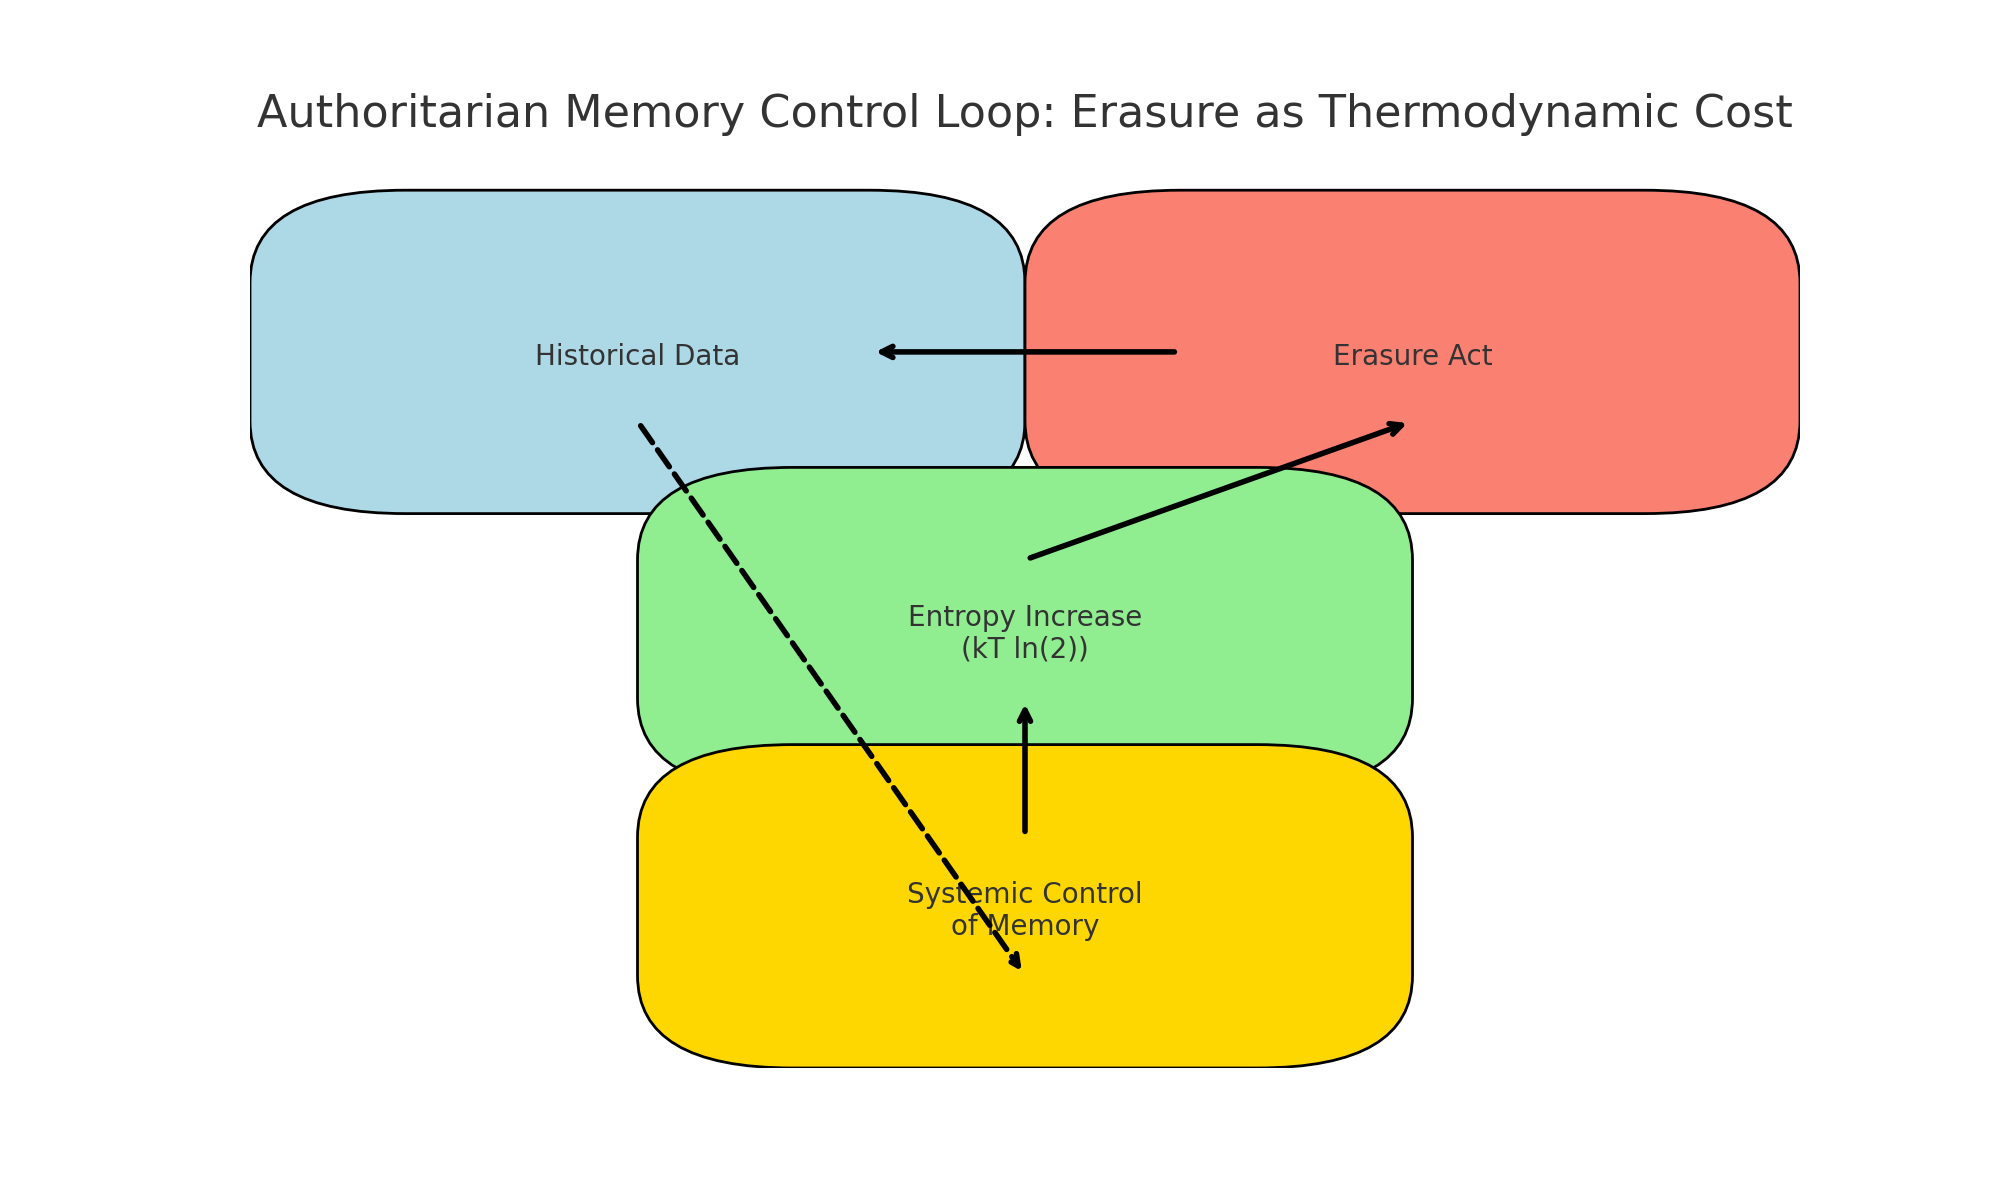
\includegraphics[width=0.8\textwidth]{assets/entropy_erasure_feedback.png}
\caption{Authoritarian memory control loop: erasure of historical data as a thermodynamic act.}
\end{figure}

\begin{center}\rule{0.5\linewidth}{0.5pt}\end{center}

\emph{Note: This section was adapted from a reflection shared in the
following conversation:
\url{https://chatgpt.com/share/e/686a11b8-f908-8009-80af-64ccb1d0798b}.
It will be integrated into the Collapse Algorithm book, cross-referenced
with the chapters on surveillance capitalism, thermodynamic entropy, and
historical revisionism.}
